\documentclass[12pt, a4paper]{extreport}
\usepackage[
margin=0.7in
]{geometry}
\usepackage[onehalfspacing]{setspace}
\usepackage[T1]{fontenc}
\usepackage{times}
\usepackage[zswash,lite, subscriptcorrection]{mtpro2}
\DeclareMathSymbol{0}{\mathalpha}{operators}{`0}
\DeclareMathSymbol{1}{\mathalpha}{operators}{`1}
\DeclareMathSymbol{2}{\mathalpha}{operators}{`2}
\DeclareMathSymbol{3}{\mathalpha}{operators}{`3}
\DeclareMathSymbol{4}{\mathalpha}{operators}{`4}
\DeclareMathSymbol{5}{\mathalpha}{operators}{`5}
\DeclareMathSymbol{6}{\mathalpha}{operators}{`6}
\DeclareMathSymbol{7}{\mathalpha}{operators}{`7}
\DeclareMathSymbol{8}{\mathalpha}{operators}{`8}
\DeclareMathSymbol{9}{\mathalpha}{operators}{`9}
\usepackage{nccmath}
\usepackage{lipsum}
\usepackage{tikz}
\usetikzlibrary{decorations.markings}
\usetikzlibrary{arrows.meta}
\usetikzlibrary{hobby, bending}

\tikzset{
	mydash/.style={dashed, dash pattern=on 6pt off 2pt},
	arrow inside/.style={
		postaction={
			decorate,
			decoration={
				markings,
				mark=at position {#1*\pgfdecoratedpathlength-0.15cm} with {\coordinate (bent arrow 1);},
				mark=at position {#1*\pgfdecoratedpathlength-0.05cm} with {\coordinate (bent arrow 2);},
				mark=at position {#1*\pgfdecoratedpathlength+0.05cm} with {\coordinate (bent arrow 3);},
				mark=at position {#1*\pgfdecoratedpathlength+0.15cm} with {
					\coordinate (bent arrow 4);
					\draw[-{Triangle[length=3mm, width=1.6mm, bend]}] 
					(bent arrow 1) to[curve through={(bent arrow 2) .. (bent arrow 3)}] (bent arrow 4);
				}
			}
		}
	}
}

\newcounter{myfig}
\makeatletter
\newcommand{\myfig}[1][]{
	\refstepcounter{myfig}
	\textbf{FIGURE \themyfig}
	\ifx\@empty#1\@empty
	\else
	\\[-5pt]#1.
	\fi
}
\makeatother
\newcommand{\FIGURE}[1]{\hspace*{20pt}\parbox[b]{3cm}{\myfig[#1]}\\}

\begin{document}
	
	
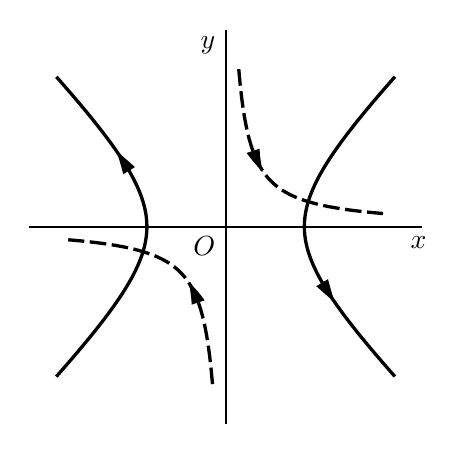
\begin{tikzpicture}[thick]
	\draw (-2.5, 0) -- (2.5, 0) node[below, pos=0.99]{$x$};
	\draw (0, -2.5) -- (0, 2.5) node[left, pos=0.96]{$y$};
	\node[below left] at (0, 0) {$O$};
	\draw[very thick,mydash, arrow inside=0.4] plot[domain=1/6:2, samples=100]({\x}, {1/(3*\x)});
	\draw[very thick,mydash, arrow inside=0.4] plot[domain=-1/6:-2, samples=100]({\x}, {1/(3*\x)});
	\draw[very thick, arrow inside=0.7] plot[domain=-1.4:1.4, samples=100]({-cosh(\x)}, {sinh(\x)});
	\draw[very thick, arrow inside=0.7] plot[domain=-1.4:1.4, samples=100]({cosh(\x)}, {-sinh(\x)});
\end{tikzpicture}\qquad
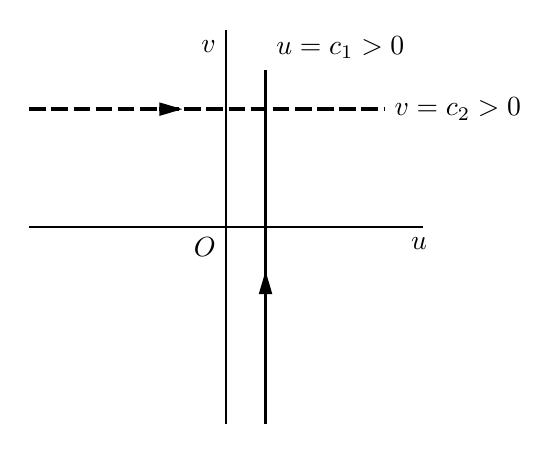
\begin{tikzpicture}[thick]
	\draw (-2.5, 0) -- (2.5, 0) node[below, pos=0.99]{$u$};
	\draw (0, -2.5) -- (0, 2.5) node[left, pos=0.96]{$v$};
	\node[below left] at (0, 0) {$O$};
	
	\draw[mydash, very thick, arrow inside=0.4] (-2.5, 1.5) -- (2, 1.5) node[right]{$v = c_2 > 0$};
	
	\draw[very thick, arrow inside=0.4] (0.5, -2.5) -- (.5, 2) node[above right]{$u=c_1>0$};
\end{tikzpicture}
\FIGURE{$w = z^2$}


%	\begin{tikzpicture}
%		\draw[thick] (0, 0) -- (4, 0);
%		
%		\draw[thick] (0, 0) -- (0, 4);
%		\draw[ultra thick] (0, 0) -- (3, 0);
%		\draw[ultra thick] (0, 0) -- (0, 3);
%		\draw[arrow inside=0.7, arrow inside=0.9, red, thick, domain=1/3:3, samples=100] plot({\x}, {1/\x});
%
%		\draw[ultra thick, arrow inside=0.2, arrow inside=0.55] (2,0) arc(0:360:2);
%	\end{tikzpicture}

%\begin{figure}[ht]
%\noindent
	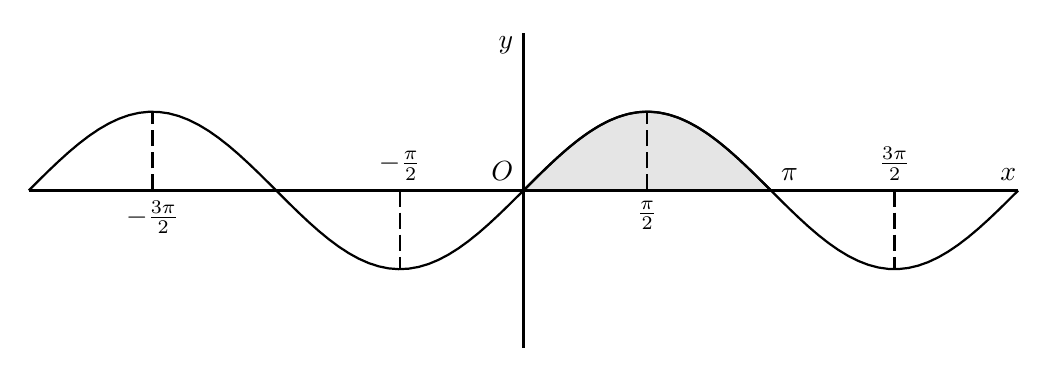
\begin{tikzpicture}[scale=1, thick]
	\draw[fill=black!10,domain=0:pi, samples=100] plot({\x}, {sin(\x r)});
	\draw[domain=-2*pi:2*pi, samples=100] plot({\x}, {sin(\x r)});
	\draw (-2*pi, 0) -- (2*pi, 0) node[above, pos=0.99]{$x$};
	\draw (0, -2) -- (0, 2) node[left, pos=0.96]{$y$};
	\node[above left] (0, 0) {$O$};
	\node[above right] at (pi, 0) {$\pi$};
	\node[below] at (pi/2, 0) {$\frac{\pi}{2}$};
	\node[above] at (-pi/2, 0) {$-\frac{\pi}{2}$};
	\node[above] at (3*pi/2, 0) {$\frac{3\pi}{2}$};
	\node[below] at (-3*pi/2, 0) {$-\frac{3\pi}{2}$};
	\draw[mydash] (pi/2, 0) -- (pi/2, 1);
	\draw[mydash] (-pi/2, 0) -- (-pi/2, -1);
	\draw[mydash] (3*pi/2, 0) -- (3*pi/2, -1);
	\draw[mydash] (-3*pi/2, 0) -- (-3*pi/2, 1);
\end{tikzpicture}
\FIGURE{$y = \sin x$}

%\begin{figure}[ht]
%\noindent
	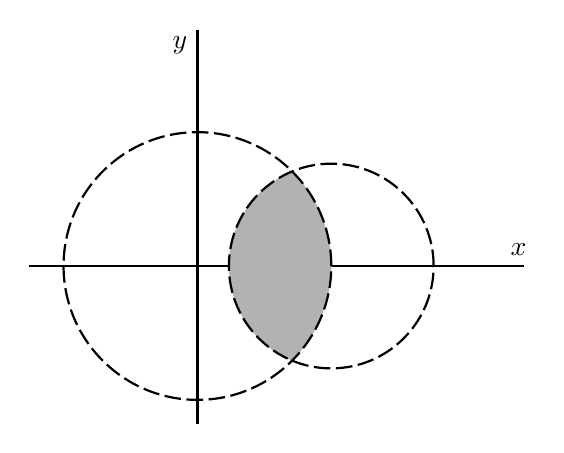
\begin{tikzpicture}[scale=1,thick]
		\draw (-pi+1, 0) -- (pi+1, 0) node[above, pos=0.99]{$x$};
		\draw (0, -2) -- (0, 3) node[left, pos=0.96]{$y$};
%		\node[above left] (0, 0) {$O$};
		
		\begin{scope}
			\clip (0,0) circle(1.7);
			\fill[black!30] (1.7,0) circle(1.3);
		\end{scope}
%		\begin{scope}
%			\clip (0,0) circle(1);            % Restrict to left circle
%			\fill[blue!20]                    % Fill only area outside overlap
%			[even odd rule]
%			(0,0) circle(1)
%			(1,1) circle(1);
%		\end{scope}
%		
%		% Right circle minus left (red)
%		\begin{scope}
%			\clip (1,1) circle(1);            % Restrict to right circle
%			\fill[red!20]
%			[even odd rule]
%			(1,1) circle(1)
%			(0,0) circle(1);
%		\end{scope}
		
		\draw[mydash] (0, 0) circle (1.7);
		\draw[mydash] (1.7, 0) circle (1.3);
	\end{tikzpicture}
	\FIGURE{Interaction}

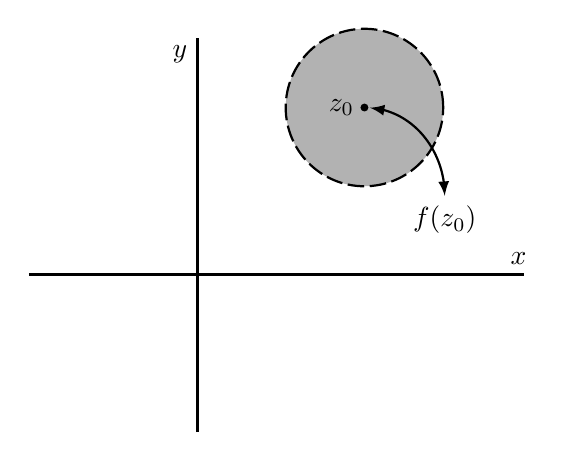
\begin{tikzpicture}[scale=1, thick]
	\draw (-pi+1, 0) -- (pi+1, 0) node[above, pos=0.99]{$x$};
	\draw (0, -2) -- (0, 3) node[left, pos=0.96]{$y$};
	\coordinate (A) at (45:3);
	\draw[mydash, fill=black!30] (A) circle (1);
	\draw[fill=black] (A) circle (1pt) node[left]{$z_0$};
	\draw[latex-latex, shorten >=2pt] (pi, 1) to[out=90, in=0] (A);
	\node[below] at (pi, 1) {$f(z_0)$};
\end{tikzpicture}
\FIGURE{}

\begin{tikzpicture}[scale=1, thick]
	\draw (-pi+1, 0) -- (pi+1, 0) node[above, pos=0.99]{$x$};
	\draw (0, -2) -- (0, 3) node[left, pos=0.96]{$y$};
	\coordinate (A) at (70:2);
	\draw[fill=black] (A) circle (2pt) node[right]{$z = x+iy$};
	\draw[-latex, 
	shorten >=3pt, very thick
	] (0:0) -- (A);
	\draw (0:.3) arc(0:90:.3 and .4);
	\draw (90:.4) arc(90:180:.5 and .4);
	\draw (180:.5) arc(180:270:.5 and .6);
	\draw (270:.6) arc(270:360:.7 and .6);
	\draw[-latex] (0:.7) arc(0:69:.7) node[right, pos=0.55]{$\theta$};
\end{tikzpicture}
\FIGURE{}

\begin{tikzpicture}[scale=12,thick]
	\draw (-0.5, 0) -- (1, 0) node[below, pos=0.99]{$x$};
	\draw (0, -1/4) -- (0, 1/4) node[left, pos=0.96]{$y$};
	
	\draw[very thick, arrow inside/.list={0.8}] plot[domain=0.1:1, samples=300]({\x},{(\x*\x*\x*sin(pi/\x r)});
\end{tikzpicture}
\FIGURE{}

{\noindent
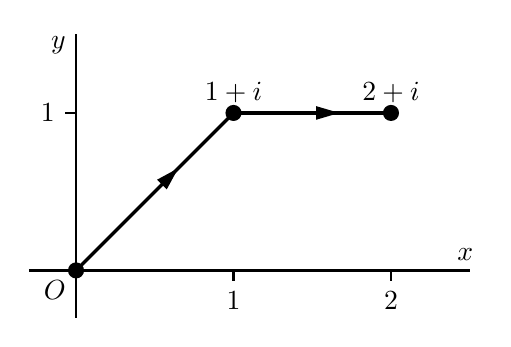
\begin{tikzpicture}[scale=2, thick]
	\draw (-0.3, 0) -- (2.5, 0) node[above, pos=0.99]{$x$};
	\draw (0, -0.3) -- (0, 1.5) node[left, pos=0.96]{$y$};
	\coordinate (A) at (0, 0);
	\coordinate (B) at (1, 1);
	\coordinate (C) at (2, 1);
	\draw[fill=black] (A) circle (1.25pt) node[below left]{$O$};
	\draw[fill=black] (B) circle (1.25pt) node[above]{$1+i$};
	\draw[fill=black] (C) circle (1.25pt) node[above]{$2+i$};
	\draw[thick] (0, 1) -- (-0.07, 1) node[left]{$1$};
	\draw (1, 0) -- (1, -.07) node[below]{$1$};
	\draw (2, 0) -- (2, -.07) node[below]{$2$};
	\draw[very thick, arrow inside=0.6] (A) -- (B);
	\draw[very thick, arrow inside=0.6] (B) -- (C);
\end{tikzpicture}
\FIGURE{}}

{\noindent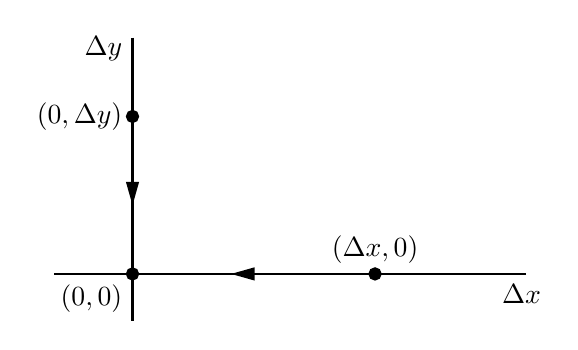
\begin{tikzpicture}[thick, scale=2]
	\draw[arrow inside=0.6] (2.5, 0) -- (-0.5, 0) node[below, pos=0.01]{$\Delta x$};
	\draw[arrow inside=0.55]  (0, 1.5) -- (0, -0.3) node[left, pos=0.04]{$\Delta y$};
	\draw[fill=black] (0, 0) circle (1pt) node[below left]{$(0, 0)$};
	\draw[fill=black] (0, 1) circle (1pt) node[left]{$(0, \Delta y)$};
	\draw[fill=black] (1.54, 0) circle (1pt) node[above]{$(\Delta x, 0)$};
\end{tikzpicture}
\FIGURE{}}

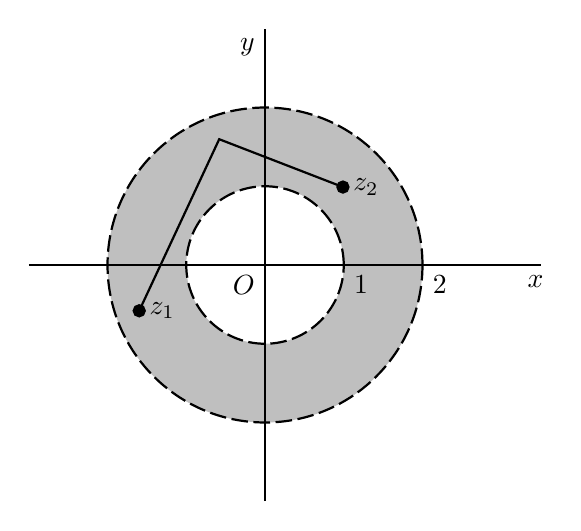
\begin{tikzpicture}[thick]
	\draw[mydash, fill=gray!50] (0, 0) circle (2);
	\draw[mydash, fill=white] (0, 0) circle (1);
	
	\draw (-3, 0) -- (3.5, 0) node[below, pos=0.99]{$x$};
	\draw (0, -3) -- (0, 3) node[left, pos=0.96]{$y$};
	\node[below left] at (0, 0) {$O$};
	\node[below right] at (1, 0) {$1$};
	\node[below right] at (2, 0) {$2$};
	
	\coordinate (z1) at (45:1.4);
	\coordinate (z2) at (200:1.7);
	
	\draw[fill=black] (z1) circle (2pt) node[right]{$z_2$};
	\draw[fill=black] (z2) circle (2pt) node[right]{$z_1$};
	\draw (z1) -- (110:1.7) -- (z2);
\end{tikzpicture}
\FIGURE{}


\end{document}